\chapter{Design}
\label{cha:design}
This chapter details the overall design of the system to be developed in this project. The software engineering methodology to be used will first be discussed, along with use cases, requirements and the architecture of the system. This will be followed up with notes on the class and database design diagrams. The decisions made with regards to some design choices will also be discussed in more detail.

\section{Methodology}
The software engineering methodology used in developing an application can have many effects on its final outcome. The development of this system will be carried out using principles taken from continuous integration and agile methods such as feature-driven development. There is always a working code repository available for deployment, and all new features to be implemented are to be worked on in clones of said repository. Upon completion of these minor implementations, they are tested to ensure everything is working correctly and assuming there are no issues, the changes are merged into the base repository. This methodology assures developers that if any major issues arise due to recent changes, they will be able to discard all changes and restart if they feel debugging would be a longer process. This ultimately allows for a faster development cycle and provides rigorous testing throughout the implementation process. This development methodology also allows for frequently changing requirements which is to be expected in any development task.

\section{Use Cases}
\label{sec:uc}
There are two main use cases for the proposed system. The following use case definitions apply only to the first stage of the system, i.e. retrieving and storing posts from Twitter. In both cases the system requirements converge, and will be explored below.

\subsection[Use Case 1]{UC1 - Streaming Twitter}
The first use case for the system requires a tool capable of continuously monitoring public tweets and storing these in a database. These tweets should be filtered by language and relevance, that is, tweets should be related to software. These tweets need to be filtered by language to counter any issues faced in the feature extraction stage due to the complexities involved in NLP. This use case will thus be referred to as streaming Twitter as that is its principle aim.

\subsection[Use Case 2]{UC2 - Searching Twitter}
The second use case for the proposed system requires the ability to search Twitter for tweets concerning user-specified key terms, and as such will henceforth be referred to as searching Twitter. These key terms should also be related to software. The returned tweets will also be filtered by language as in the streaming use case to counter the NLP complexities. An extra function required here should be to see which software tools have been mentioned most often, and these should be displayed to the users with the option to search again, or see the full analysis of these tools.


\subsection{Merging the Use Cases}
Upon fulfilling these core requirements, the systems should store these tweets in a database for work in the remaining stages. The first of these is extracting the previously stated features from these tweets. These features must again be stored separately from the initial tweet data, as some tweets may contain information regarding more than one piece of software. Finally, all of this information must be aggregated and shown to users in the form of charts displaying sentiment, and all relevant information found alongside it.

% MAY NEED UC DIAGRAMS

\section{General Architecture}
As previously explained, the system design follows a 3-stage approach, these being tweet retrieval, feature extraction and visualisation for users. These stages are shown in the general archicture model displayed in Figure~\ref{fig:general}. These will be further explored in Sections~\ref{sec:arc1}, \ref{sec:arc2} and \ref{sec:arc3} respectively.

\begin{figure}[h]
\begin{center}
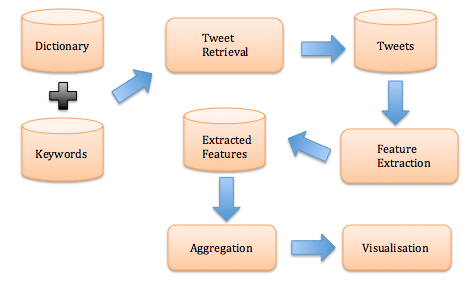
\includegraphics[width=12cm]{design}
\end{center}
\caption{General architecture of the system}
\label{fig:general}
\end{figure}

\subsection{Retrieving Tweets}
\label{sec:arc1}
The first stage involves retrieving tweets from Twitter. The design for this stage follows the same concepts for each of the use cases defined. This can then be split further as seen in Figure~\ref{fig:phase1}. The program should retrieve a set of search terms from a dictionary along with some keywords that may be associated with software. These are to be used to form a request for tweets from Twitter. Twitter will respond with the corresponding tweets and data, which are to be checked for language, to ensure they are in English. The remaining set of English tweets are then to be further parsed to extract the required information for storing these tweets in the database.

\begin{figure}[h]
  \centering
  \setlength{\unitlength}{0.0125in}
\begin{picture}(300,35)(95,730)
\thicklines
\put(0,740){\framebox(75,20){Filter terms}}
\put(75,750){\vector( 1, 0){ 20}}
\put(95,740){\framebox(75,20){Twitter API}}
\put(170,750){\vector( 1, 0){ 20}}
\put(190,740){\framebox(110,20){Language detection}}
\put(300,750){\vector( 1, 0){ 20}}
\put(320,740){\framebox(80,20){Parse response}}
\put(400,750){\vector( 1, 0){ 20}}
\put(420,740){\framebox(75,20){Store in DB}}
\end{picture}

  \caption{Design for tweet retrieval
    \label{fig:phase1}}
\end{figure}

This returned information will be stored in a relational database and its design is shown below in Figure~\ref{fig:db}. Tweets will not be stored alone but also with simple user information to allow for future user profiling for a more targetted approach to tweet retrieval. The actual tweet information to be stored is its id on the Twitter platform - allowing for cases where users delete their tweets - its text content, time of creation, user id and the keyword used to find it, where one was used. There will also be fields for sentiment, i.e. positive, negative or neutral, and sentiment strength, where weightings have been used. These fields should default to \texttt{NULL} as their values will be computed at a later time. Finally, there is a \emph{tagged} boolean flag which signifies the given tweet has been processed, and the feature extraction process has been carried out on it. This is to be implemented in MySQL due to its simplicity, compatibility with the design and also because it is readily available on the university computers where data can be easily accessed both locally and remotely.

\begin{figure}[h]
\begin{center}
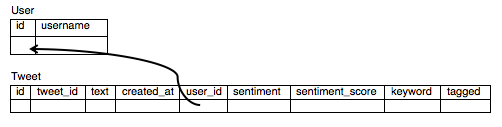
\includegraphics[width=12cm]{db}
\end{center}
\caption{Database design for storing tweets}
\label{fig:db}
\end{figure}

\subsection{Feature Extraction}
\label{sec:arc2}
The feature extraction stage will execute the task of extracting information from tweets. This will involve the stages described in \ref{sec:textmining} and its general design can be seen in Figure~\ref{fig:phase2}. The main aim of this stage is to take the tweets previously stored in the database and find the softwares mentioned in them.

\begin{figure}[h]
  \centering
  \setlength{\unitlength}{0.0125in}
\begin{picture}(300,200)( 50, 0)
\thicklines
\put(0,140){\framebox(110,20){Sentiment analysis}}
\put(110,150){\vector( 1, 0){ 20}}
\put(130,140){\framebox(100,20){URL extraction}}
\put(170,750){\line( 1, 0){ 10}}
\put(180,750){\line(0,-1){50}}

\put(300,750){\vector( 1, 0){ 20}}
\put(400,750){\vector( 1, 0){ 20}}



\put(130,140){\framebox(100,20){Price extraction}}
\put(130,140){\framebox(100,20){POS Tagging}}
\put(130,140){\framebox(100,20){Main features}}
\put(130,140){\framebox(100,20){Verify software}}


\end{picture}

  \caption{Design for feature extraction
    \label{fig:phase2}}
\end{figure}

Due to the volatile nature of the information being extracted from these tweets, this data should be stored in a NoSQL-type database, that is, a schema-less design that diverges from the traditional relational database model. As a result, there is no formal design for this database structure, however, it is required of the system to at this stage store any features it has managed to extract along with the key information associated with the tweet that had been stored in the tweet retrieval stage, such as its unique id and text content.

\subsection{Visualisation}
\label{sec:arc3}
The visualisation stage has the task of displaying all the gained information and knowledge to the user. Ultimately, it must also provide a graphical interface for users to interact with the system in order to perform their own searches.

There are two parts to this phase of project. Firstly, the data gathered must be \emph{aggregated} so that meaningful knowledge can ultimately be represented. Upon completing this task, a \emph{graphical user interface} (GUI) must be designed for users to interact with the system, perform their own queries, and look at what information has been found.

\subsection{Aggregation}
Aggregating the results is the process of bringing together all the different data sources for data on a single output entity such as a piece of software. This aggregated data can then be used easily by the GUI to display understandable information to the user.

\subsection[Graphical User Interface]{Graphical User Interface (GUI)}
The GUI of choice is a web application as opposed to a desktop application, as it allows for a more centralised system that users can easily connect to. It is also a more scalable solution as updates would not need to be pushed out to all users.


% WIRE FRAMES?

